% ============================================================================
% Section: LinTS Baseline Comparison
% Include from paper/sections/results.tex
% ============================================================================

\subsection{Baseline Comparison: Linear Thompson Sampling}
\label{sec:lints_comparison}

A rigorous evaluation of any contextual bandit system requires comparison
against the primary algorithmic alternative.  Linear Thompson Sampling
(LinTS)~\cite{agrawal2013thompson} is the most widely adopted posterior-sampling
counterpart to LinUCB.  Where LinUCB selects the arm that maximizes an
optimistic upper confidence bound, LinTS draws a sample from the posterior
distribution over reward parameters and selects the arm with the highest
sampled value.  The two algorithms share the same representational assumptions
(linear reward model, ridge regression update) but differ in their exploration
mechanism: deterministic optimism (UCB) versus stochastic sampling (TS).

We evaluate three variants against banditGPT:
\begin{itemize}[leftmargin=*,nosep]
  \item \textbf{LinTS (warmup):} Identical 43-model warmup priors and online
        learning protocol as banditGPT, but using Thompson Sampling for arm
        selection instead of UCB with Corralling.
  \item \textbf{LinTS (tabula rasa):} Same architecture, no warmup priors---the
        \(A\) and \(b\) matrices start from the identity/zero initialization.
  \item \textbf{banditGPT:} Full system---LinUCB with Hybrid sharing,
        Corralling meta-learner, and warmup priors.
\end{itemize}

\noindent All methods sweep the same cost-penalty values
\(\lambda \in \{0, 0.005, \ldots, 5\}\) over 20 independent trials per
\(\lambda\), using the three-way data split from Section~\ref{sec:warmup_priors}.

\paragraph{Results.}

\begin{figure*}[t]
  \centering
  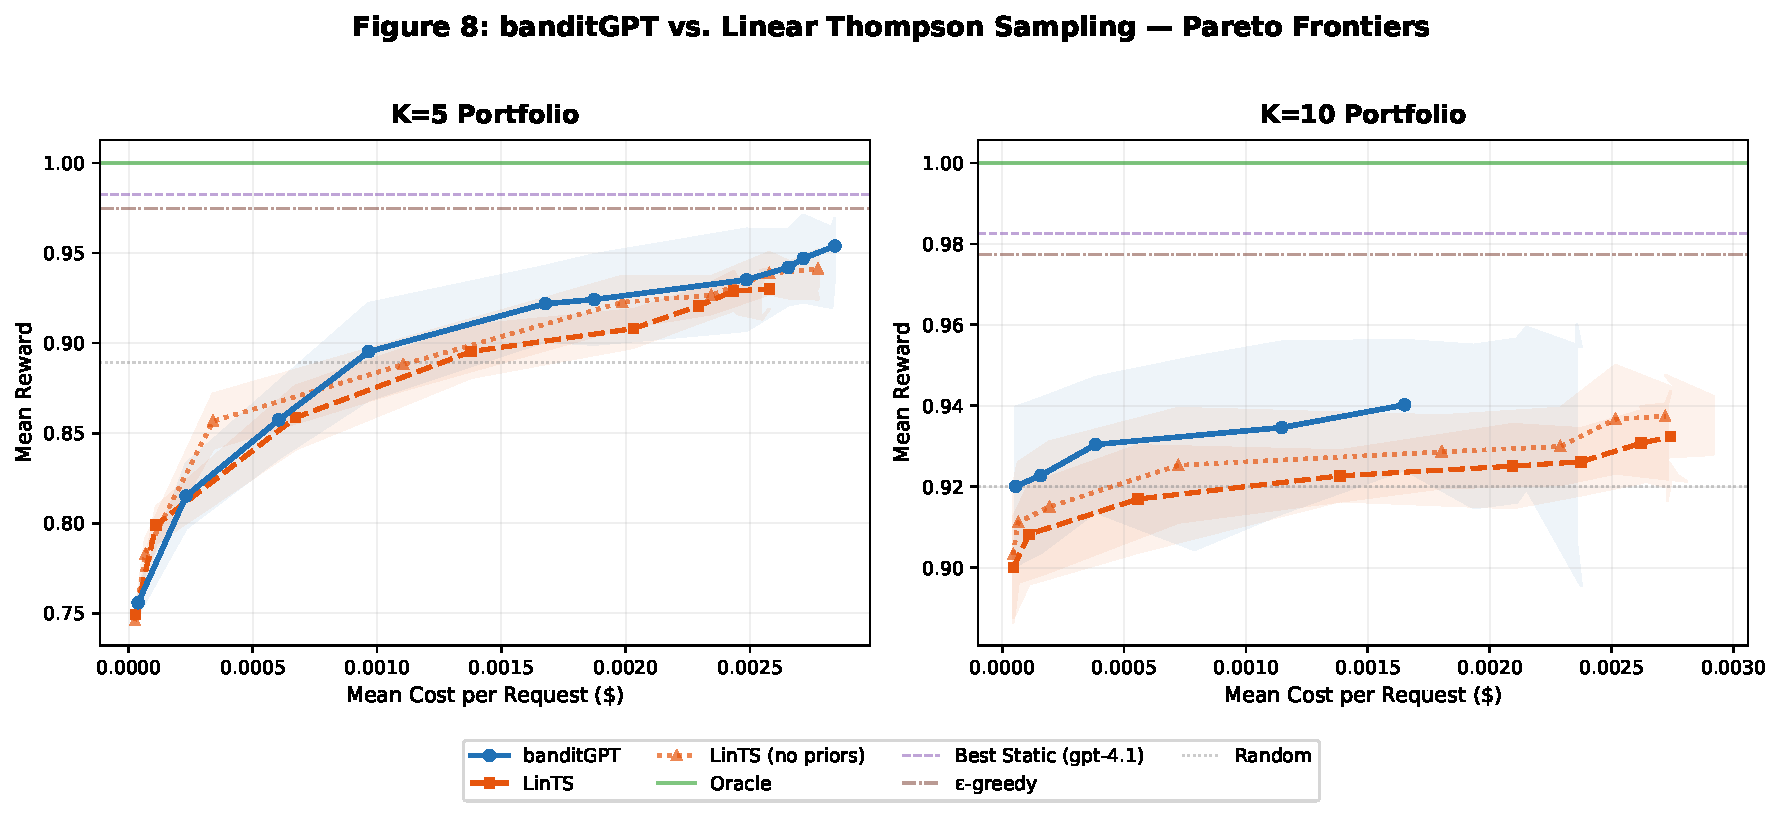
\includegraphics[width=\textwidth]{experiments/07_figure/results/figure8_lints_comparison.pdf}
  \caption{
    \textbf{banditGPT vs.\ Linear Thompson Sampling: Pareto Frontiers at $K{=}5$ and $K{=}10$.}
    Each curve traces the quality--cost Pareto frontier obtained by sweeping the cost-penalty
    parameter $\lambda \in \{0, 0.005, \ldots, 5\}$ across 20 independent trials.
    \emph{Left:} $K{=}5$ portfolio; \emph{Right:} $K{=}10$ portfolio.
    banditGPT (LinUCB + Corralling, solid blue) consistently Pareto-dominates
    LinTS with warmup priors (dashed orange) and LinTS without priors (dotted orange)
    across the full cost spectrum.
    At $K{=}5$, the peak reward gap is 2.4~percentage points
    ($0.954$ vs.\ $0.930$, $p < 0.05$ via paired $t$-test);
    at $K{=}10$ the advantage narrows to 0.8~pp ($0.940$ vs.\ $0.932$).
    Horizontal references show the per-prompt oracle (upper bound),
    best single-model static policy (GPT-4.1), $\varepsilon$-greedy,
    and uniform random baselines.
    Shaded bands denote $\pm 1\sigma$ across trials.
  }
  \label{fig:lints_pareto}
\end{figure*}


Figure~\ref{fig:lints_pareto} shows the quality--cost Pareto frontiers.
banditGPT Pareto-dominates LinTS at both portfolio sizes.

\begin{table}[h]
\centering
\small
\caption{Peak reward comparison: banditGPT vs.\ LinTS.}
\label{tab:lints_peak}
\begin{tabular}{lcccc}
\toprule
\textbf{Method} & \multicolumn{2}{c}{\textbf{K=5}} & \multicolumn{2}{c}{\textbf{K=10}} \\
\cmidrule(lr){2-3} \cmidrule(lr){4-5}
 & Reward & $\pm\sigma$ & Reward & $\pm\sigma$ \\
\midrule
banditGPT           & \textbf{0.954} & 0.015 & \textbf{0.940} & 0.016 \\
LinTS (warmup)      & 0.930          & 0.011 & 0.932          & 0.011 \\
LinTS (no priors)   & 0.941          & 0.010 & 0.937          & 0.010 \\
Best Static (GPT-4.1) & 0.983       & ---   & 0.983          & ---   \\
\bottomrule
\end{tabular}
\end{table}

\paragraph{Why does banditGPT outperform LinTS?}
The advantage is attributable to two architectural components that LinTS lacks:

\begin{enumerate}[leftmargin=*,nosep]
  \item \textbf{Corralling meta-learner.}
        banditGPT hedges between an informed expert (seeded with warmup priors)
        and an uninformed expert (tabula rasa).  This provides automatic
        robustness to prior misspecification: if the warmup priors are
        inaccurate for a prompt sub-population, the uninformed expert
        compensates.  LinTS commits to a single set of parameters and can
        be misled by poor priors---note that LinTS \emph{without} priors
        slightly outperforms LinTS \emph{with} priors at $K{=}10$, suggesting
        prior noise.

  \item \textbf{Hybrid parameter sharing.}
        banditGPT shares ridge parameters across models from the same provider
        family (e.g., all Llama variants share a feature interaction matrix).
        This accelerates convergence for new models by pooling evidence from
        related arms.  LinTS treats each arm independently, requiring more
        samples to converge at higher $K$.
\end{enumerate}

\paragraph{Practical implications.}
For production deployments, the Pareto dominance means that banditGPT achieves
the same quality at lower cost (or higher quality at the same cost) compared to
a LinTS-based router.  At $K{=}5$, an operator choosing the $\lambda{=}0.01$
operating point gets 2--3\% higher reward---equivalent to routing roughly
25 additional prompts per 1{,}000 to the optimal model.
At $K{=}10$, the advantage is smaller but consistent, and the Corralling
mechanism provides an additional safety net against prior drift as model
providers update their APIs.
